\chapter{Concept and Implementation}
\label{chapter:conceptApproachSolution}

\section{Methodology}

To investigate the usefulness of the integration of biological knowledge in FS for gene expression data, we developed a framework for the comparison of computational, knowledge based and combined FS methods. 
The framework is depicted in Fig. \ref{fig:framework}.
The inputs of the framework are a labeled dataset and an external knowledge base.
The outputs of it are ranked lists of features from computational, knowledge based and combined methods as well as evaluation results for how well the different methods perform.
It is divided into the three independent steps of
\begin{enumerate*}[label={\alph*)},font={\bfseries}]
    \item feature selection,
    \item feature combination and
    \item feature evaluation.
\end{enumerate*}

\begin{figure}[h!]
\setlength{\belowcaptionskip}{-15pt}
\centering
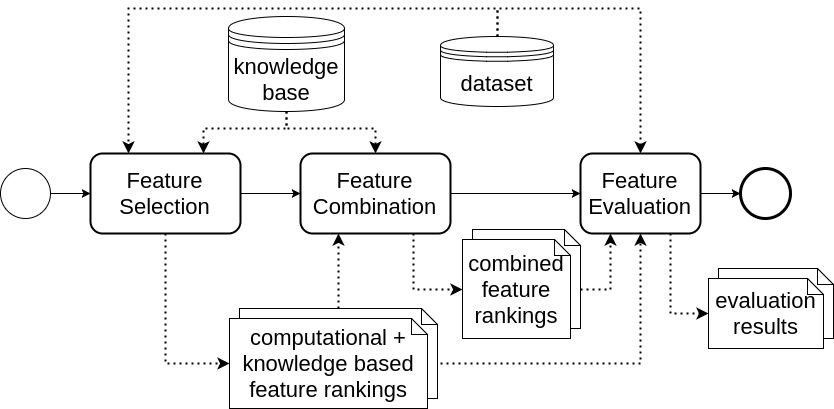
\includegraphics[width=0.95\textwidth]{figures/architecture2.png}
\caption{Three step integrative feature selection, combination and evaluation framework}
\label{fig:framework}
\end{figure}

\subsection{Feature Selection} 

The feature selection step takes a dataset and information from prior knowledge as inputs and can be further divided into the application of computational FS techniques and our knowledge based FS approach. 
It outputs computational and knowledge based feature rankings.

Firstly, the computational FS part takes the dataset and produces feature rankings using statistical or machine learning based methods.  
Secondly, the knowledge based FS approach creates a feature ranking by accessing the API of the knowledge base DisGeNET which integrates data from different scientific biological sources\cite{pinero2015disgenet}.
This database contains information on $>$ 17 K genes and $>$ 20 K diseases with $>$ 560 K gene-disease-associations (GDAs).
DisGeNET scores the GDAs by their level of evidence. 
The DisGeNET feature ranking is produced by
\begin{enumerate*}[label={\alph*)},font={\bfseries}]
    \item extracting a list of diseases from the dataset,
    \item fetching a list of genes for each disease that are sorted by their GDA score,
    \item filtering these lists by a user-defined top \emph{k} or threshold value and
    \item combining all lists into one.
\end{enumerate*}
The last step, i.e. the combination of the gene lists for the diseases, is done by interleaving. 
This way we prevent diseases with genes that have high association scores to dominate the gene ranking and allow each disease to be represented equally in the gene ranking.

\subsection{Feature Combination} 

The feature combination step uses the produced feature rankings as well as prior knowledge as inputs and returns combined feature rankings. 
As shown in the example depiction in Fig. \ref{fig:combination}, our approach filters the computational feature rankings by keeping only genes that biological knowledge identified as connected to the diseases apparent in the dataset. 

\begin{figure}[h!]
\setlength{\belowcaptionskip}{-15pt}
\centering
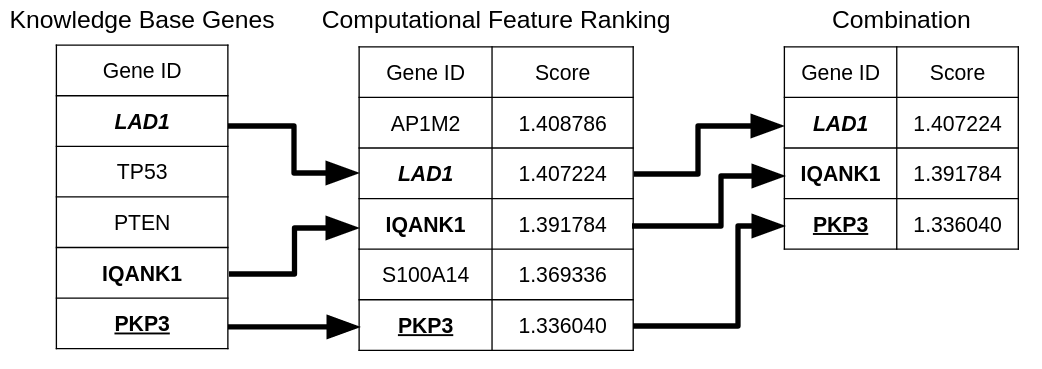
\includegraphics[width=0.95\textwidth]{figures/combination3.png}
\caption{Combination feature ranking by using knowledge base extracted genes as a filter for the computational feature ranking}
\label{fig:combination}
\end{figure}

We use DisGeNET and KEGG as knowledge bases in this step.
For DisGeNET, we use all genes contained in the DisGeNET feature ranking as an unranked set of genes.
For KEGG, we use all genes that are contained in pathways connected to the diseases extracted from the dataset.

\subsection{Feature Evaluation}

This step takes the dataset as well as all previously produced feature rankings as inputs and outputs evaluation results for them.
From each ranking, only the top \emph{n} features are retained where \emph{n} starts with 2 and increases to 100. 
With the dataset reduced to the selected set of features, the user can choose between multiple different classifiers for training and evaluation. 
A classification performance metric that is averaged over those classifiers is reported in order to compare classifier-independent performance.

\subsection{Technical Implementation}

We integrate WEKA\cite{hall2009weka} and R in our framework for maximum flexibility regarding selecting FS methods and classifiers and metrics for evaluation. 
Therefore, Java and R are used for the feature selection and only Java for the feature evaluation.
The integration of external knowledge is implemented by accessing their APIs using python.
The framework itself and the feature combination step is implemented in python, too.

\section{Mathematical Model}
\label{subsec:mathModel}

Mathmatical Model.

\section{Architecture}

Architecture.
